\section*{Appendix I: On Phase Singularities}

To construct the expression for an isolated optical vortex, we start from the wave equation
\begin{eqnarray}
	&&c^2\nabla^2\psi = \frac{\partial^2 \psi}{\partial t^2}.
	\label{eq:wave}
\end{eqnarray}
One can verify that wave functions of the form
\begin{eqnarray}
	&&\psi = (a + b\textcolor{blue}{y}) e^{i(kz - \omega t)}
	\label{eqn_301}
\end{eqnarray}
which are waves with linearly modulated amplitude, satisfy Eq. (\ref{eq:wave}). 
Now we consider two primary wave trains, say wave $A$ and $B$, assuming that they are monochromatic and modulated linearly along $y$-direction so that one rises, as the other falls. 
If wave $A$ and $B$ coincide with each other on the $y = 0$ plane with an angle $2 \alpha$ (see Fig. \ref{fig:two_primary_waves}), one can write down their wave expression
\begin{eqnarray}
	&&\psi_A = a_0(1 + \beta k_1 y) e^{i(k_1 x + k_3 z - \omega t - \pi/2)}
	\nonumber \\
	&&\psi_B = a_0(1 - \beta k_1 y) e^{i(-k_1 x + k_3 z - \omega t + \pi/2)}
	\label{eqn_302}
\end{eqnarray}
\textcolor{red}{Draw a schematic to represent $\psi_A$ and $\psi_B$.
	Resosolve the inconsistency between $\psi_A$, $\psi_B$ in (\ref{eqn_302}) and $\psi$ in (\ref{eqn_301}).}
where $\bar{k} = \hat{x} k_1 + \hat{z} k_3$ is the propagating vector of wave $A$, 
$a_0$ and $\beta$ are constants representing the amplitudes of carrier and modulating waves, respectively.

\begin{figure}[h]
	\vskip 6 cm
	\hskip 0.3 cm
	\special{wmf: primary_waves.pdf x=7 cm y=6 cm}
	\caption{Illustration for the primary waves $A$ and $B$.}
	\label{fig:two_primary_waves}
\end{figure}
%\begin{figure}[h]
%	\centering
%	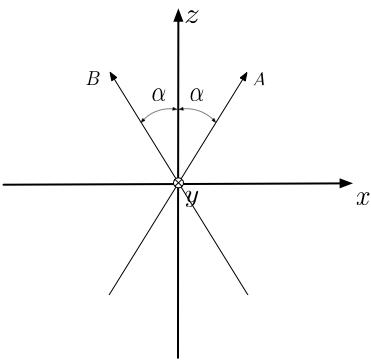
\includegraphics[width = 0.4\textwidth]{primary_waves.jpg}
%	\caption{Illustration for the primary waves $A$ and $B$.}
%	\label{fig:two_primary_waves}
%\end{figure}

Let $c = \omega/k$, $k_1 = k \sin \alpha$, $k_3 = k \cos \alpha$, $\xi = k_1 x$, $\zeta = k_3 z - \omega t$ and $\eta = k_1 y$. 
The resultant complex wave field can be represented by the superposition of $A$ and $B$,
\begin{eqnarray}
	&&\psi = \psi_A + \psi_B = a_0 \left[ ( 1 + \beta \eta ) e^{i(\xi + \zeta - \pi/2)} \right. 
	\nonumber\\
	&&\hspace{0.3in} \left. + ( 1 - \beta \eta ) e^{i (- \xi + \zeta + \pi/2)} \right]
	\nonumber\\
	&&= 2 a_0 e^{i\zeta} \left[ \cos(\xi - \pi/2) + i \beta \eta \sin(\xi - \pi/2) \right]
	\nonumber\\
	&&= 2 a_0 e^{i\zeta} \left( \sin \xi - i \beta \eta \cos\xi \right)
	\nonumber
\end{eqnarray}
Therefore we can explicitly write down the formula of the wave in complex forms, \textcolor{blue}{$\psi = |\psi| e^{i\Phi}$,}
\textcolor{red}{What are $\rho$ and $\Phi$?}
\begin{eqnarray}
	&&\textcolor{blue}{|\psi|^2} = 4a_0^2 (\sin^2 \xi + \beta^2 \eta^2 \cos^2 \xi)
	\nonumber\\
	&&\Phi = 2n\pi + \zeta - \arctan\left(\frac{\beta \eta}{\tan \xi} \right).
\end{eqnarray}
Now, put $A_0 = 2a_0 \sin\alpha$ and let $\alpha \rightarrow 0$ without changing $A_0$ and $k$,
\begin{eqnarray}
	&&\textcolor{blue}{|\psi|^2} = A_0^2 \left[ \frac{\sin^2 (k\sin\alpha)x}{\sin\alpha^2} + \beta^2 k^2 y^2 \cos^2(k\sin\alpha)x \right]
	\nonumber\\
	&& \hspace{0.15in} \rightarrow A_0^2\left( k^2 x^2 + \beta^2 k^2 y^2 \right)
\end{eqnarray}
and
\begin{eqnarray}
	&&\Phi = 2n\pi + \left[(k \cos\alpha) z - \omega t \right] - \arctan\left(\frac{\beta \eta}{\tan \xi} \right)
	\nonumber\\
	&& \hspace{0.15in} \rightarrow 2n\pi + (kz - \omega t) - \arctan\left(\beta y/ x\right).
	\label{eq:limit}
\end{eqnarray}

Set $\beta = 1$ and represent Eq. (\ref{eq:limit}) in cylindrical coordinates, i.e. $(r, \phi, z)$ with $r^2 = x^2 + y^2, \phi = \arctan(y/x), z = z$,
\begin{eqnarray}
	\psi(r, \phi, z) = A_0 kr e^{i(k z - \omega t - \phi)}.
	\label{eq:single_vortex}
\end{eqnarray}
Eq. (\ref{eq:single_vortex}) characterizes an isolated skew-dislocation \cite{Ber73} of ``strength'' $m = 1$.

Having established the method to find the equation for a skew-dislocation by mixing two primary waves and performing a limiting process, Nye and Berry \cite{Ber73} claimed that these field expressions can be guessed \emph{a priori}. Therefore we need only generalize the present complex wave function $\psi$ we already have and keep they still satisfy the wave equation Eq. (\ref{eq:wave}). By this, we shall interpret the yielded functions as representing various kinds of dislocations, namely vortices.

In this perspective, Eq. (\ref{eq:single_vortex}) can be extended to the form
\begin{eqnarray}
	\psi = \left[ Ar^m + \left( \frac{B}{r^m} \right)\right] e^{i(kz - \omega t \pm m \phi)},
	\label{eq:vortex_m}
\end{eqnarray}
which still complies with Eq. (\ref{eq:wave}). Eq. (\ref{eq:vortex_m}) describes vortices with strength, or more precisely, topological charge, equals $m$. To define the topological charge, we consider a closed curve $C$ in the $(\bar{r}, t)$-space and perform the following steps:
\begin{enumerate}
	\item Around the curve $C$ the phase angle $\Phi$ may undergo a change of $2n \pi$, with $n \in {\cal Z}$ and $n \neq 0$.
	\item Shrink the closed curve $C$ to an arbitrarily small loop without changing $n$.
	\item If such a curve $C$ can be found, then $C$ is claimed to enclose a singularity because $\Phi$ varies infinitely fast 
	around the center point.
	\item The smoothness of the function $\psi$ implies that this scenario can only happen at points where $\psi = 0$, where $\Phi$ is not well-defined.
\end{enumerate}
A winding number $S_C$, characterizing the strength of this singularity, is defined as 
\begin{eqnarray}
	S_C = \frac{1}{2 \pi} \oint_C d \Phi = \frac{1}{2 \pi} \oint_C \nabla \Phi \cdot d \bar{r}
\end{eqnarray}
where $C$ is a contour enclosing the singularity.

\section*{Appendix II: 2-D Fourier Transformation of Vortex Beam}
To compute the counterpart in frequency domain of the field $U(r, \phi, 0) = e^{i\phi}$, we recall the Fourier transformation pair
\begin{eqnarray}
	A(\nu_x, \nu_y, z) = \int_{-\infty}^{\infty} \int_{-\infty}^{\infty} U(x, y, z)
	e^{-i 2 \pi (\nu_x x + \nu_y y)} dx dy
	\nonumber\\
	U(x, y, z) = \int_{-\infty}^{\infty} \int_{-\infty}^{\infty} A(\nu_x, \nu_y, z)
	e^{i 2 \pi (\nu_x x + \nu_y y)} d\nu_x d\nu_y.
	\nonumber
\end{eqnarray}
Perform the following change of variable:
\begin{eqnarray}
	x = r\cos\phi & y = r\sin\phi & r \ge 0, 0 \le \phi \le 2\pi
	\nonumber\\
	\nu_x = \rho\cos\chi & \nu_y = \rho\sin\chi & \rho \ge 0, 0 \le \chi \le 2\pi
	\nonumber
\end{eqnarray}
Thus, we have
\begin{eqnarray}
	&&dx dy = r dr d\phi, \hspace{0.1in} d\nu_x d\nu_y = \rho d\rho d\chi,
	\nonumber\\
	&&x\nu_x + y\nu_y = r\rho \cos(\phi - \chi).
	\nonumber
\end{eqnarray}
To sum up, the 2-D Fourier transformation pair in cylindrical coordinate is represented by
\begin{eqnarray}
	A(\rho, \chi, z) = \int_{0}^{2\pi} \int_{0}^{\infty} U(r, \phi, z)
	e^{-i 2 \pi r \rho \cos(\phi - \chi)} r dr d\phi
	\nonumber\\
	U(r, \phi, z) = \int_{0}^{2\pi} \int_{0}^{\infty} A(\rho, \chi, z)
	e^{i 2 \pi r \rho \cos(\phi - \chi)} \rho d\rho d\chi.
	\nonumber
\end{eqnarray}

Therefore, one can compute ${\cal F} \{e^{i\phi}\}$ as follows:
\begin{eqnarray}
	&&A(\rho, \chi, 0) = \int_{0}^{2\pi} e^{i\phi} 
	\left(\int_{0}^{\infty} e^{-i2\pi \rho r \cos(\phi - \chi)} r dr\right) d\phi
	\nonumber\\
	&&\hspace{0.5in}= \int_{0}^{2\pi} \frac{-e^{i\phi}}{4 \pi^2 \rho^2 \cos^2(\phi - \chi)} d\phi
	\nonumber\\
	&&\hspace{0.5in}= \frac{1}{\pi^2 \rho^2} \int_{0}^{2\pi} \frac{-e^{i\phi} d\phi}{e^{i(\phi - \chi)} + e^{-i(\phi - \chi)}}
	\nonumber\\
	&&\hspace{0.5in}= \frac{ e^{i\chi} }{\pi^2 \rho^2} \int_{\chi}^{\chi + 2\pi}
	\frac{-e^{i\phi'} d\phi'}{e^{i\phi'} + e^{-i\phi'}},
	\hspace{0.1in} (\phi' = \phi - \chi)
	\nonumber\\
	&&\hspace{0.5in}= \frac{i e^{i \chi}}{\pi^2 \rho^2} \oint_C \frac{dz}{(z + z^{-1})^2}
	\nonumber\\
	&&\hspace{0.5in}= \frac{i e^{i \chi}}{\pi^2 \rho^2} \oint_C \frac{z^2 dz}{(z^2 + 1)^2},
\end{eqnarray}
where the last complex contour integration is performed counterclockwise along the boundary $C$ of unit circle centered at the origin. Since the integrand in the last equality has two poles of order $2$ located at $i$ and $-i$ (both are on $C$), respectively, the contour integration can only be defined by Cauchy principal value, i.e.
\begin{eqnarray}
	{\cal P} \oint_C \frac{z^2 dz}{(z^2 + 1)^2} = \lim_{\epsilon \rightarrow 0} \oint_{C_{\epsilon}} \frac{z^2 dz}{(z^2 + 1)^2},
	\label{eq:CPV}
\end{eqnarray}
where $C_{\epsilon}$ is a curve defined as Fig. \ref{fig:contour}.

\begin{figure}[h]
	\vskip 6 cm
	\hskip 0.3 cm
	\special{wmf: contour.pdf x=7 cm y=6 cm}
	\caption{Contour of $C_{\epsilon}$.}
	\label{fig:contour}
\end{figure}
%\begin{figure}
%	\centering
%	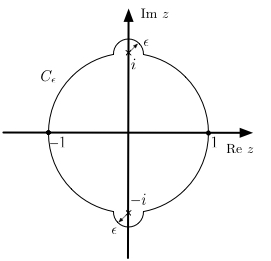
\includegraphics[width = .4\textwidth]{contour.jpg}
%	\caption{Contour of $C_{\epsilon}$, which is formed by the boundary of the union of the unit circle centered at the origin and two circles with radius $\epsilon$ centered at $i, -i$, repectively.}
%	\label{fig:contour}
%\end{figure}
Note that $C_{\epsilon} \rightarrow C$ as $\epsilon \rightarrow 0$. The contour integration on $C_{\epsilon}$, on the other hand, can be evaluated by residue theorem.
\begin{eqnarray}
	\oint_{C_{\epsilon}} \frac{z^2}{(z^2 + 1)^2} = 2\pi i \left( {\rm Res}(f; i) + {\rm Res}(f; -i) \right),
	\label{eq:thm_residue}
\end{eqnarray}
with $f$ denoting the integrand in Eq. (\ref{eq:CPV}). By invoking the identity ${\rm Res}(f; a) = 1/(n-1)! \lim_{z \rightarrow a} d^n (z - a)^n f(z) /dz^n$ for a pole $a$ of order $n$, the residues can be computed:
\begin{eqnarray}
	{\rm Res}(f; i) = 1/8, & {\rm Res}(f; -i) = 3/8.
	\nonumber
\end{eqnarray}
Hence, Eq. (\ref{eq:thm_residue}) yields
\begin{eqnarray}
	A(\rho, \chi, 0) = \frac{- e^{i \chi}}{\pi \rho^2}. (?)
\end{eqnarray}

\section*{Appendix III: Paraxial Wave Eqation}
\label{sec:pwe}
Given a monochromatic electromagnetic field $\tilde{U}(x, y, z) \exp(-i \omega t) = U(x, y, z)\exp[i (kz - \omega t)]$, we have known that it satisfies the Helmholtz equation
\begin{eqnarray}
	\left(\nabla^2 + k^2\right) \tilde{U}(x, y, z) = 0.
	\label{eq:helmholtz}
\end{eqnarray}
If we compute
\begin{eqnarray}
	\frac{\partial^2}{\partial z^2} U(x, y, z)e^{ikz} = e^{ikz}
	\left( \frac{\partial^2 U}{\partial z^2} + 2ik \frac{\partial U}{\partial z} - k^2 U \right),
	\nonumber
\end{eqnarray}
Then Eq. (\ref{eq:helmholtz}) becomes
\begin{eqnarray}
	\left(\frac{\partial^2}{\partial x^2} + \frac{\partial^2}{\partial y^2} + \frac{\partial^2}{\partial z^2} + 2ik \frac{\partial}{\partial z} \right) U(x, y, z) = 0
	\label{eq:helmholtz_2}
\end{eqnarray}
One can further simplify the equation by performing {\em the paraxial approximation}:
\begin{eqnarray}
	\left| \frac{\partial^2 U}{\partial z^2} \right| \ll \left| 2k \frac{\partial U}{\partial z} \right|,
	\label{eq:paraxial}
\end{eqnarray}
which can be interpreted physically that the variation along $z$-axis is so small that all of the light must travel nearly paralle to the $z$-axis. Therefore, Eq. (\ref{eq:helmholtz_2}) is reduced to
\begin{eqnarray}
	\left(\nabla_{\perp}^2 + 2ik \frac{\partial}{\partial z} \right) U(x, y, z) = 0.
	\label{eq:pwe}
\end{eqnarray}
Usually, laser beams satisfy the paraxial approximation (\ref{eq:paraxial}) very well, whence it is convenient to model them by Eq. (\ref{eq:pwe}).

\section*{Appendix IV: Fast Fourier Transform}

Let $u(x)$ be a single-variable function of $x$.
In order to perform DFT suitably, the function $U$ must have a bounded support, namely,
$u(x) = 0$ unless $|x| \leq L_x$, where $L_x$ is a finite number.
Otherwise, the function $u(x)$ must be truncated such that $u(x) \neq 0$ only if $0 \leq x \leq L_x$. 

Consider $N$ equispaced samples at $x = n \Delta x$, where $\Delta x = L_x / N$.
Thus, $u (x)$ is sampled to form a sequence $\{ u[n] \}$, with
\begin{eqnarray}
	&&u [n] = u (x = n \Delta x)
	\nonumber
\end{eqnarray}
The Fourier transform of $u(x)$ is discretized as
\begin{eqnarray}
	&&\hspace{-0.3in} U (\nu) = \int_{-\infty}^{\infty} u (x) e^{- i 2 \pi \nu x} dx
	\simeq \Delta x \sum_{n = 0}^{N - 1} u (n \Delta x) e^{- i 2 \pi \nu n \Delta x}
	\nonumber
\end{eqnarray}
The spectrum is also discretized as
\begin{eqnarray}
	&&\hspace{-0.3in} U[m] = U (m \Delta \nu) \simeq \Delta x \sum_{n = 0}^{N - 1} u [n] e^{- i 2 \pi m \Delta \nu n \Delta x}
	\label{eqn_3041}
\end{eqnarray}
By demanding the uncertainty principle that $\Delta \nu \Delta x =  1/N$,
(\ref{eqn_3041}) is reduced to
\begin{eqnarray}
	&&U[m] \simeq \Delta x \sum_{n = 0}^{N - 1} u [n] e^{- i 2 \pi m n / N}
	\label{eqn_3042}
\end{eqnarray}
which can be implemented as
\begin{eqnarray}
	&&U[m] = \Delta x {\rm FFT} \{ u [n] \}
	\label{eqn_3042a}
\end{eqnarray}

Similarly, the inverse Fourier transform of $U (\nu)$ is discretized as
\begin{eqnarray}
	&&\hspace{-0.3in} u(x) = \int_{-\infty}^{\infty} U (\nu) e^{i 2 \pi \nu x} d \nu
	\simeq \Delta \nu \sum_{m = 0}^{N - 1} U (m \Delta \nu) e^{i 2 \pi m \Delta \nu x}
	\nonumber
\end{eqnarray}
which is discretized as
\begin{eqnarray}
	&&u[n] = u(n \Delta x) 
	\simeq \Delta \nu \sum_{m = 0}^{N - 1} U [m] e^{i 2 \pi m \Delta \nu n \Delta x} 
	\nonumber \\
	&&= \frac{1}{N \Delta x} \sum_{m = 0}^{N - 1} U [m] e^{i 2 \pi m n /N} 
	\label{eqn_3043}
\end{eqnarray}
which can be implemented as
\begin{eqnarray}
	&&u[n] = \frac{1}{\Delta x} {\rm IFFT} \{ U [m] \}
	\label{eqn_3043a}
\end{eqnarray}

In MATLAB, the FFT and the IFFT are defined as
\begin{eqnarray}
	&&A[m] = \sum_{n = 0}^{N - 1} a[n] e^{-i 2\pi m n/ N}
	\nonumber \\
	&&a[n] = \frac{1}{N} \sum_{m = 0}^{N - 1} A[m] e^{i 2 \pi mn/N}.
	\label{eq:DFT_pairs}
\end{eqnarray}

\section*{Appendix V: Gaussian Beam and Laguerre-Gaussian modes}
\subsection{Fundamental Gaussian beam}
Recalling the paraxial wave equation (PWE, Eq. (\ref{eq:pwe})) introduced in Section \ref{sec:pwe}, now we set out to find an important family of solutions to it.

We proceed by trials. Suppose a function $\tilde{U}(r, z) = U(r, z) e^{i k z}$ satisfies Eq. (\ref{eq:pwe}), where $U(r, z)$ takes the form
\begin{eqnarray}
	U(r,  z) = e^{i [ P(z) + kr^2/2q(z)]}
	\label{eq:gb_trial}
\end{eqnarray}
for some undetermined $P(z)$ and $q(z)$ satisfies Eq. (\ref{eq:pwe}), where $r^2 = x^2 + y^2$.  Writing PWE in cylindrical coordinates
\begin{eqnarray}
	\left[ \frac{1}{r} \frac{\partial}{\partial r} \left( r \frac{\partial}{\partial r}\right) + 2ik \frac{\partial}{\partial z} \right] U(r, \phi, z) = 0
\end{eqnarray}
and substituting Eq. (\ref{eq:gb_trial}) into, we will have
\begin{eqnarray}
	&& \frac{1}{r} \frac{\partial}{\partial r} \left( r \frac{\partial}{\partial r}\right) U
	= \frac{1}{r} \frac{\partial}{\partial r} \left( \frac{ i k r^2}{q} U \right)
	\nonumber\\
	&&\hspace{0.5in} = \frac{1}{r} \left[ \frac{2 i k r}{q} U + \left( \frac{i k r^2}{q}\right)
	\frac{\partial U}{\partial r} \right]
	\nonumber\\
	&&\hspace{0.5in} = U \left[ \frac{2 i k }{q} 
	+ \left( \frac{i k r}{q} \right) \left( \frac{ i k r}{q} \right) \right]
	\nonumber\\
	&&\hspace{0.5in} = U \left( \frac{2 i k }{q} - \frac{k^2 r^2}{q^2} \right) 
\end{eqnarray}
and
\begin{eqnarray}
	&& 2ik \frac{\partial U}{\partial z} = 2ik U \left( i \frac{\partial P}{\partial z}
	- i \frac{k r^2}{2 q^2} \frac{\partial q}{\partial z} \right)
	\nonumber\\
	&&\hspace{0.5in} = U \left( -2k \frac{\partial P}{\partial z} + \frac{k^2 r^2}{q^2} 
	\frac{\partial q}{\partial z} \right),
\end{eqnarray}
and finally
\begin{eqnarray}
	&& \left[ \frac{1}{r} \frac{\partial}{\partial r} \left( r \frac{\partial}{\partial r}\right) + 2ik \frac{\partial}{\partial z} \right] U
	\nonumber\\
	&&\hspace{0.5in} = U \left[ 2k \left( \frac{i}{q} - \frac{\partial P}{\partial z} \right)
	+ \frac{k^2 r^2}{q^2} \left( \frac{\partial q}{\partial z} - 1 \right) \right] = 0.
	\nonumber
\end{eqnarray}
To determine $P$ and $q$, we solve the system
\begin{eqnarray}
	&&\frac{\partial q}{\partial z} = 1,
	\label{eq:pwe_q}\\
	&&\frac{\partial P}{\partial z} = \frac{i}{q}.
	\label{eq:pwe_P}
\end{eqnarray}
By demanding the integration constant to be pure imaginary, the solution to Eq. (\ref{eq:pwe_q}) is represented as
\begin{eqnarray}
	q(z) = z - i z_0
\end{eqnarray}
for some real constant $z_0$, which is know as {\em Rayleigh range}. Eq. (\ref{eq:pwe_P}) can therefore be solved as
\begin{eqnarray}
	P(z) = i \ln (1 + i \frac{z}{z_0}),
\end{eqnarray}
where we have used the initial condition $P(0) = 0$. Putting all pieces together, we will end up with
\begin{eqnarray}
	U(r, z) = \frac{1}{\sqrt{1 + (z/z_0)^2}} e^{-i\tan^{-1} (z/z_0)} 
	e^{\frac{-k z_0 r^2 + i k z r^2}{2(z^2 + z_0^2)}}.
	\label{eq:gb_z}
\end{eqnarray}
At this point we can define some important parameters
\begin{eqnarray}
	&& W_0 = \sqrt{\lambda z_0/\pi},
	\nonumber\\
	&& W(z) = W_0 \sqrt{1 + (z/z_0)^2},
	\nonumber\\
	&& R(z) = z(1 + (z_0/z)^2),
	\nonumber\\
	&& \zeta(z) = \tan^{-1}(z/z_0),
	\nonumber
\end{eqnarray}
where $W_0$ is the beam waist, $W(z)$ is the measure of beam width, $R(z)$ represents the wavefront radius of curvature, and $\zeta(z)$ is called the {\em Gouy phase shift}. Hence, Eq. (\ref{eq:gb_z}) becomes
\begin{eqnarray}
	U(r, z) = \frac{W_0}{W(z)} e^{-r^2/W^2(z)} e^{i k r^2/ 2 R(z)} e^{-i \zeta(z)}.
	\nonumber
\end{eqnarray}
Putting back the $e^{ikz}$ term, we obtain the expression for fundamental Gaussian beam
\begin{eqnarray}
	&& \tilde{U}(r, z) = U(r, z) e^{ikz}
	\nonumber\\
	&& \hspace{0.3in} = \frac{W_0}{W(z)} e^{-r^2/W^2(z)} e^{i k r^2/ 2 R(z)} e^{i (kz - \zeta(z))}.
	\label{eq:gb}
\end{eqnarray}
\textcolor{blue}{
For convenience, we will refer to Eq. (\ref{eq:gb}) by $\tilde{U}_0 = U_0 e^{ikz}$ in the following context.
}

\subsection{Laguerre-Gaussian modes}
In order to take the orbital angular momentan (OAM) presented by vortices into acounts, one need not only the fundamental Gaussian mode but a higher order family derived from it. Similarly, one can pick out reasonable trials from what we have already learned in the derivation of Gaussian beams and check the necessary conditions for them to satisfy paraxial wave equation (\ref{eq:pwe}). In Appendix I we have briefly investigated the nature of vortices, which are skrew-dislocations and characterized by a helical phase term $e^{i m \phi}$, so it is tempting to consider if the function $U_0 e^{im \phi}$, where $U_0$ is the fundamental Gaussian beam, satisfies PWE. Unfortunately, this can not achieve the goal due to appearance of extra terms. Another plausible option is
\begin{eqnarray}
	U(r, \phi, z) = U_0 S(r) e^{i m \theta}.
	\label{eq:trial_lag_gb}
\end{eqnarray}
This trial, however, will be shown to result in a set of solutions to PWE called Laguerre-Gaussian modes.

By substituing Eq. (\ref{eq:trial_lag_gb}) in to PWE, one will have
\begin{eqnarray}
	&&\left(\nabla_{\perp}^2 + 2 i k \frac{\partial}{\partial z}\right) U(r, \phi, z)
	\nonumber\\
	&& \hspace{0.3in} = U_0 e^{i m \phi} \left[ \frac{d^2 S}{d r^2} + 
		\left( \frac{2 i k r}{q} + \frac{1}{r} \right) \frac{d S}{d r} 
			- \frac{m^2}{r^2} S \right].
	\nonumber
\end{eqnarray}
Thus the unknown function $S(r)$ can be determined by solving the ordinary differential equation
\begin{eqnarray}
	S'' + \left( \frac{2 i k r}{q} + \frac{1}{r} \right) S' - \frac{m^2}{r^2} S = 0.
\end{eqnarray}

\textcolor{magenta}{If we perform the transformation and change of variable
\begin{eqnarray}
	&&S(r) = \left(\frac{\sqrt{2}r}{W(z)}\right)^{m} \tilde{S}(r),
	\nonumber\\
	&&r^2 = \frac{W^2(z)}{2} u,
	\nonumber
\end{eqnarray}
the ODE becomes
\begin{eqnarray}
	u \tilde{S}''(u) + (m + 1 - p)\tilde{S}'(u) + p\tilde{S}(u) = 0,
\end{eqnarray}
which is the Laguerre differential equation and has the solution
\begin{eqnarray}
	\tilde{S}(u) = L_{pm}(u),
\end{eqnarray}
where $L_{pm}(u)$ is the generalized Laguerre polynomial. In summary, the solution can be represented by
\begin{eqnarray}
	&&U^{p}_{m}(r, \phi, z)
	\nonumber\\
	&&= \frac{W_0}{W(z)} \left(\frac{\sqrt{2} r}{W(z)}\right)^{m} L_{pm}\left(\frac{2 r^2}{W^2(z)}\right)
	\nonumber\\
	&&\hspace{0.5in} e^{-r^2/W^2(z)}  e^{i \left[k r^2/ 2 R(z) + kz - \zeta(z) + m \phi\right]}.
\end{eqnarray}}

\textcolor{blue}{
Another appoarch to obtain the expression for Laguerre-Gaussian modes is by Fresnel's diffraction theory under the paraxial assumption, which is equivalent to our angular spectrum method (except that evanescent components of the spectrum plays no role under paraxial approximation). According to the theory, the complex amplitude wave function after propagation over $z$ can be reprsented by the convolution of field distribution at $z = 0$ with the Fresnel kernel $h(x, y, z) = (1 / i \lambda z) \exp(ik(x^2 + y^2)/2z)$. Since Fresnel diffraction integral has assumed paraxial condition, the result derived will still satisfy PWE as long as the initial aperture field does.
}

\textcolor{blue}{
One can check the function
\begin{eqnarray}
	U_{m}^{p}(r, \phi, 0) = C_{mp} L^{|m|}_{p}\left( \frac{2r^2}{W_0^2} \right)
		e^{-r^2/W_0^2} e^{i m \phi}
\end{eqnarray}
will indeed satisfy PWE Eq. (\ref{eq:pwe}). By carrying out the integral in Cartesian coordinates,
\begin{eqnarray}
	U_{m}^{p}(x, y, z) = \frac{1}{i \lambda z} \int_{-\infty}^{\infty} \int_{-\infty}^{\infty}
		U_{m}^{p}(x_0, y_0, 0) \times
	\nonumber\\
	e^{ik[(x - x_0)^2 + (y - y_0)^2]/2z} dx_0 dy_0,
\end{eqnarray}
finally one will obtain
\begin{eqnarray}
	U_{m}^{p}(r, \phi, z) = \frac{C_{mp}}{W} \left(\frac{\sqrt{2} r}{W}\right)^{|m|}
		e^{-r^2/W^2} L^{|m|}_{p}\left( \frac{2r^2}{W^2} \right) \times
	\nonumber\\
	e^{i(2p + m + 1)\zeta + i kr^2/2R} e^{im\phi},
\end{eqnarray}
where $C_{mp}$ is a normalization constant represented by
\begin{eqnarray}
	C_{mp} = \sqrt{\frac{2p!}{\pi (p + |m|)!}}.
\end{eqnarray}}

\textcolor{blue}{
\section*{Appendix VI: Simulation and Testing}
In this section, we will simulate the near-core structure with the approach in Section \ref{sec:angular_spectrum}
and Fig.\ref{fig:commu_diag}. 
We will start from the wave expression for the Laguerre-Gaussian ${\rm LG}^{0}_{1}$ mode, which is characterized by an optical vortex of strength $1$ at the center.
The field of ${\rm LG}^{0}_{1}$ vortex beam is represented at $z = 0$ as
\begin{eqnarray}
U(r, \phi, 0) = \frac{2r}{\sqrt{\pi} W_0^2} e^{-r^2/W_0^2} e^{i\phi} 
\end{eqnarray}
}

%\begin{eqnarray}
%	&&\phi(x, y) = \left\{
%	\begin{array}{ll}
%		\tan^{-1}(y/x), & x > 0 \\ & \\
%		\tan^{-1}(y/x) + \pi, & x < 0, y > 0 \\ & \\
%		\tan^{-1}(y/x) - \pi, & x < 0, y < 0 \\ & \\
%		(\pi/2) {\rm sign}(y), & {\rm otherwise}
%	\end{array}
%	\right.
%\end{eqnarray}
%where 
%\begin{eqnarray}
%	{\rm sign}(y) = \left\{
%	\begin{array}{ll}
%		1, \hspace{0.2in}	& y > 0 \\ & \\
%		-1,		& y < 0 \\ & \\
%		0,		& y = 0
%	\end{array}
%	\right.
%\end{eqnarray}

\textcolor{blue}{In the simulations, He-Ne laser with $\lambda = 633$ nm is chosen as the light source.
The aperture is confined to $L_0 \times L_0$ in the $xy$ plane, with $L_0 = 10 \mu$m.
The beam waist is taken to be $W_0 = 0.388$ mm, and the corresponding Rayleigh range is $z_0 = \pi W_0^2/ \lambda \simeq 0.75$ m \cite{FSM05}.
The aperture length $L_0$ is sampled at $N = 1,024$ uniformly spaced points, in the $x$ and $y$ directions, 
with intervals $\Delta x = \Delta y = L_0 / N$.
The corresponding intervals in the spectral domain are $\Delta \nu_x = \Delta \nu_y = 1 / L_0$.}

The field expression after propagation over a distance of $z$ can be obtained by two appoarches. One of them is:
\begin{enumerate}
	\item Compute $A(\nu_x, \nu_y, 0) = {\cal F} \{ U(x, y, 0) \}$.
	\item Compute $\mu = -2 \pi^2 (\nu_x^2 + \nu_y^2) / k$ (obtained from paraxial approximation and dropping the $\exp(ikz)$ term).
	\item Compute $A(\nu_x, \nu_y, z) = A(\nu_x, \nu_y, 0) e^{i \mu z}$.
	\item Compute $U(x, y, z) = {\cal F}^{-1} \{A(\nu_x, \nu_y, z)\}$.
\end{enumerate}

And the other follows:
\begin{enumerate}
	\item For fixed $z$, discretize $h(x, y, z) = (1/i \lambda z) \exp[i k (x^2 + y^2) / 2z]$ along $x$ and $y$ directions.
	\item Discretize $U(x, y, 0)$.
	\item Compute $U(x, y, z) = h(x, y, z) * U(x, y, 0)$.
\end{enumerate}

After the computation of the field at $z = \lambda, 10\lambda, 100\lambda$, we plot the evolution of vortex beam and compare them with the exact solution.

%After obtaining the phase information, we plot following types of diagrams:
%\begin{enumerate}
%	\item Fix $r = 0.1 \lambda, 0.3 \lambda, 0.5\lambda, 1.0 \lambda$, and plot the relationship between the retarded phase (helical component $\exp(i \phi)$ removed) $\Phi = {\rm arg}~ U(x, y, z) - \phi$ and propagation distance $z$.
%	\item  Fix $r = 0.1 \lambda, 0.3 \lambda, 0.5 \lambda, 1.0 \lambda$, and plot the relationship between the additional phase dip $kz - \Phi$ and propagation distance $z$.
%	\item For propagation distance $z = 1\lambda, 10 \lambda, 100 \lambda$, plot the retarded phase distribution $\Phi(x, y, z)$.
%	\item For propagation distance $z = 1\lambda, 10 \lambda, 100 \lambda$, plot the total phase distribution ${\rm arg}~ U(x, y, z)$.
%\end{enumerate}